\documentclass{beamer}
%\documentclass[handout]{beamer}

\usepackage{amsmath}
\usepackage{tikz}
\usepackage{commath}

\graphicspath{{figures/}}
\DeclareGraphicsExtensions{.pdf,.png,.jpg}

\usetikzlibrary{arrows,shapes,fit,backgrounds}

\newcommand{\ev}[1]{\langle #1 \rangle} % expectation value

\title[Quantum GI]
{Distinguishing graphs with a quantum annealer
  using susceptibility measurements} 

\author[Wittmann, Hen, Young]{%
  Matthew~Wittmann\inst{1} \and
  Itay~Hen\inst{2} \and
  A.~P.~Young\inst{1}
}

\institute[UCSC and ISI]
{
  \inst{1}%
  Physics Department\\
  University of California, Santa Cruz
  \and
  \inst{2}%
  Information Sciences Institute\\
  University of Southern California
}
\date[APS MM 2014]{APS March Meeting, 2014}

\begin{document}

% TikZ commands needed for fancy equation annotation
% see http://www.texample.net/tikz/examples/beamer-arrows/
\tikzstyle{every picture}+=[remember picture]
\tikzstyle{na} = [baseline=-.5ex]
\everymath{\displaystyle}

\frame{\titlepage}

\section{Background}

\begin{frame}
  \frametitle{Graph isomorphism (GI) problem}
  Are two graphs really the same apart from the labeling of the vertices?
  \bigskip
  \begin{columns}[T]
    \column{0.27\textwidth}
    \centering
    $G$
    \column{0.27\textwidth}
    \centering
    $H$
    \column{0.27\textwidth}
    \centering
    \alert<1|handout:1>{$G \cong H$?}
    \uncover<2-|handout:2->{\alert{Yes.}
    }
  \end{columns}
  \bigskip
  \begin{columns}[c]
    \column{0.27\textwidth}
    \centering
    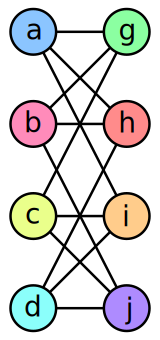
\includegraphics[scale=0.36]{Graph_isomorphism_a}

    \column{0.27\textwidth}
    \centering
    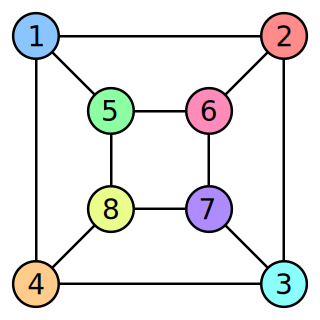
\includegraphics[scale=0.36]{Graph_isomorphism_b}

    \column{0.27\textwidth}
    \centering
    \uncover<2-|handout:2-> {%
      \begin{align*}
        a &\leftrightarrow 1 &\quad g &\leftrightarrow 5 \\
        b &\leftrightarrow 6 &\quad h &\leftrightarrow 2 \\
        c &\leftrightarrow 8 &\quad i &\leftrightarrow 4 \\
        d &\leftrightarrow 3 &\quad j &\leftrightarrow 7
      \end{align*}
    }
  \end{columns}
  \transdissolve<2>[duration=0.2]
\end{frame}

\begin{frame}
  \frametitle{Graph invariants}
  For example\ldots
  \begin{itemize}
    \item number of vertices and edges
    \item degree distribution
    \item spectrum of adjacency matrix
    \item \ldots and many more (any quantity which is invariant under
      relabeling the vertices)
  \end{itemize}
  \pause
  \begin{definition}
    An invariant $I$ is \alert{complete} if $I(G) = I(H) \iff G \cong H$.
  \end{definition}
  There are no known general, complete invariants. Finding one would provide an
  easy solution to the GI problem!
\end{frame}

\begin{frame}
  \frametitle{Complexity of the GI problem}
  \begin{columns}
    \column{0.7\textwidth}
    \begin{itemize}
      \item Special cases (e.g. trees, planar graphs) can be solved efficiently
        by classical algorithms
      \item Best known general algorithms have exponential worst-case complexity
      \item<2> Along with factoring, ``NP-incomplete''
        \tikz[na]\node [coordinate] (inpi) {};
    \end{itemize}

    \column{0.3\textwidth}
    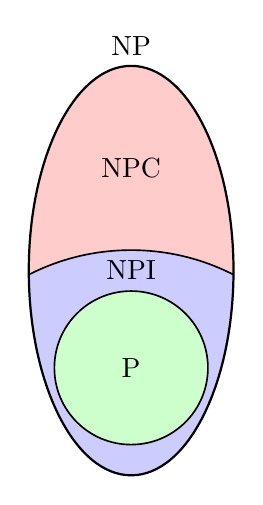
\begin{tikzpicture}[scale=1.3,semithick]
      \def\egg{(0,0) ellipse (1 and 2)}
      \fill[red!20] \egg;
      \begin{scope}[even odd rule]
        \clip\egg;
        \filldraw[fill=blue!20] (0,-2) circle (2.2);
      \end{scope}
      \filldraw[fill=green!20] (0,-0.95) circle (0.75) node {P};
      \path (0,2) node[above] {NP};
      \path (0,0.2) node[below] (npi) {NPI};
      \path (0,1) node {NPC};
      \draw[thick] \egg;
    \end{tikzpicture}
    \begin{tikzpicture}[red,overlay,semithick,>=stealth']
      \path[->]<2> (inpi) edge [out=0,in=180] (npi.west);
    \end{tikzpicture}
  \end{columns}
  \transdissolve<2>[duration=0.2]
\end{frame}

\begin{frame}
  \frametitle{GI and quantum annealing}
    \begin{columns}
      \column{0.6\textwidth}
      \begin{itemize}
        \item Hen and Young (2012):
          Propose that the GI problem could be solved using a
          quantum annealer
        \item Gaitan and Clark (2013):
          Propose adiabatic quantum algorithm for GI
        \item Vinci et al. (2013):
          Experimental implementation of GI algorithm using D-Wave quantum
          annealer
      \end{itemize}
      \column{0.4\textwidth}
      \includegraphics[width=\textwidth]{d_wave_one_system}
    \end{columns}
\end{frame}


\section{Method}

\begin{frame}
  \frametitle{Graph encoding}
  \begin{equation*}
    H_p(G) = 
    \tikz[baseline]{
      \node[fill=blue!20,ellipse,anchor=base] (afm)
      {$\sum_{(i,\,j) \in G} \sigma^z_i \sigma^z_j$};
    }
    \uncover<2->{ % only show field term starting on slide 2
      -
      \tikz[baseline]{
        \node[fill=red!20,ellipse,anchor=base] (h)
        {$h \sum \sigma^z_i$};
      }
    }
  \end{equation*}
  \begin{itemize}
    \item Antiferromagnetic Ising model
      \tikz[na]\node [coordinate] (iafm) {};
    \item<2-> Longitudinal field to break $z$-symmetry
      \tikz[na]\node [coordinate] (ih) {};
    \item<3-> Spectrum of $H_p(G)$ \alert{not} a complete invariant\ldots
  \end{itemize}
  \begin{tikzpicture}[overlay,semithick,>=stealth]
    \path[->] (iafm) edge [out=0,in=-30] (afm);
    \path[->]<2-> (ih) edge [out=0,in=-90] (h);
  \end{tikzpicture}
  \begin{definition}<3->
    $G_1,\,G_2$ \alert{co-Ising} $\iff$ $H_p(G_1)$, $H_p(G_2)$
    co-spectral for all $h$
  \end{definition}
\end{frame}

\begin{frame}
  \frametitle{Adiabatic quantum algorithm for GI}
  \begin{equation*}
    H =
    \uncover<2->{s\,}
    \tikz[baseline]{ \node[fill=blue!20,ellipse,anchor=base] (hp)
      {$H_p(G)$};
    }
    \uncover<2->{
      + (1-s)\,
      \tikz[baseline]{ \node[fill=green!20,ellipse,anchor=base] (hd)
        {$\frac{1}{2} \sum \sigma^x_i$};
      }
    }
  \end{equation*}
  \begin{itemize}[<+->]
    \item Problem Hamiltonian \tikz[na]\node [coordinate] (ihp) {};
    \item Driver Hamiltonian \tikz[na]\node [coordinate] (ihd) {};
    \item \alert{Hypothesis:} The quantum problem ($0<s<1$) will distinguish
        non-isomorphic graphs
  \end{itemize}
  \begin{tikzpicture}[overlay,semithick,>=stealth]
    \path[->] (ihp) edge [out=0,in=-45] (hp);
    \path[->]<2-> (ihd) edge [out=0,in=-90] (hd);
  \end{tikzpicture}
  \vskip -2ex
  \begin{block}{Algorithm}<+->
    \begin{enumerate}
      \item Prepare system in ground state of $H_d$ (easy)
      \item Take $s$ from 0 to 1 \alert{slowly}.  System remains in ground state
        of the instantaneous Hamiltonian (adiabatic theorem)
      \item Use measurements taken \alert{throughout the adiabatic evolution}
        to distinguish non-isomorphic graphs
    \end{enumerate}
  \end{block}
  \transdissolve<2>[duration=0.2]
\end{frame}

\begin{frame}
  \frametitle{Test case: small co-Ising graphs}
  \begin{itemize}
    \item Study pair of 13-vertex (non-isomorphic) co-Ising graphs
    \item Found to be difficult to distinguish by Vinci et al. (using
      measurements at $s \rightarrow 1$ and with $h=0$)
    \item Which $h$, $s$ give the largest difference in measured quantities?
  \end{itemize}
  \bigskip
  \begin{columns}[t]
    \column{0.5\textwidth}
    \centering
    $G_{13}$\\[1.5ex]
    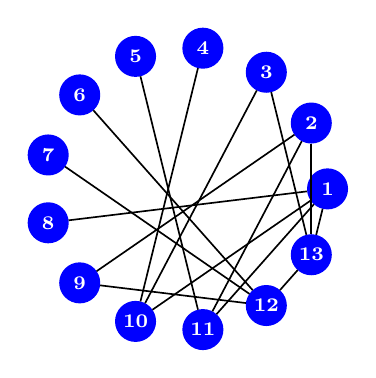
\begin{tikzpicture}[semithick]
      \tikzstyle{every node}=[circle, fill=blue, draw=blue, text=white,
        font=\scriptsize, minimum size=0.5cm, inner sep=1pt]
      \def \n {13}
      \def \radius {1.8cm}
      \foreach \s in {1,...,\n} {
        \node at ({360/\n * (\s - 1)}:\radius) (\s) {\bf\s};
      }
      \path (1)  edge (8)
                 edge (10)
                 edge (11)
                 edge (13)
            (2)  edge (9)
                 edge (11)
                 edge (13)
            (3)  edge (10)
                 edge (13)
            (4)  edge (10)
            (5)  edge (11)
            (6)  edge (12)
            (7)  edge (12)
            (9)  edge (12)
            (12) edge (13);
    \end{tikzpicture}

    \column{0.5\textwidth}
    \centering
    $G_{13}'$\\[1.5ex]
    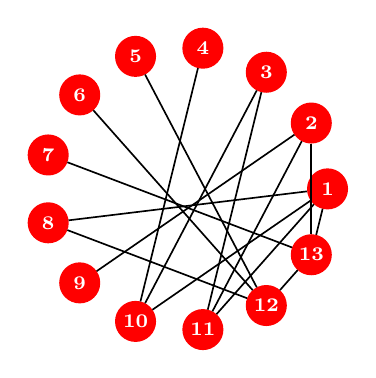
\begin{tikzpicture}[semithick]
      \tikzstyle{every node}=[circle, fill=red, draw=red, text=white,
        font=\scriptsize, minimum size=0.5cm, inner sep=1pt]
      \def \n {13}
      \def \radius {1.8cm}
      \foreach \s in {1,...,\n} {
        \node at ({360/\n * (\s - 1)}:\radius) (\s) {\bf\s};
      }
      \path (1)  edge (8)
                 edge (10)
                 edge (11)
                 edge (13)
            (2)  edge (9)
                 edge (11)
                 edge (13)
            (3)  edge (10)
                 edge (11)
            (4)  edge (10)
            (5)  edge (12)
            (6)  edge (12)
            (7)  edge (13)
            (8)  edge (12)
            (12) edge (13);
    \end{tikzpicture}
  \end{columns}
\end{frame}


\section{Results and Conclusions}

\begin{frame}
  \frametitle{Numerical results}
  \begin{center}
    Absolute value of the difference in $E_G=\ev{H_p(G)}$
    \bigskip
    \includegraphics{delta-Eg-big}
  \end{center}
\end{frame}

\begin{frame}
  \frametitle{Conclusions}
  \begin{columns}
    \column{0.5\textwidth}
    \begin{itemize}
      \item So far, it looks like graphs are distinguished by the proposed
        Ising model
      \item Differences are more pronounced in the middle of the adiabatic run
        and not at the end of it
    \end{itemize}
    \begin{block}{Future work}
      \begin{itemize}
        \item Test on D-Wave hardware capable of mid-run measurements
      \end{itemize}
    \end{block}
    
    \column{0.5\textwidth}
    \includegraphics{delta-Eg}
  \end{columns}
\end{frame}

\begin{frame}
  \frametitle{Acknowledgements}
  \begin{itemize}
    \item Co-authors Itay Hen, Peter Young
    \item Walter Vinci
    \item NASA Ames quantum group
    \item Mohammad Amin
  \end{itemize}
  \vfill
  \begin{center}
    \huge Thank you!
  \end{center}
\end{frame}

\appendix
\section{\appendixname}

\begin{frame}
  \frametitle{Measurements}
  \begin{itemize}
    \item Energies $E=\ev{H(G)}$, $E_G=\ev{H_p(G)}$
    \item Magnetizations $m_z$, $m_x$
    \item Spin glass overlap
    \begin{equation*}
      Q_2 = \frac{1}{N} \sqrt{
        \sum_{i,\,j} \del{
          \ev{\sigma^z_i \sigma^z_j} -
          \ev{\sigma^z_i} \ev{\sigma^z_j}
        }^2
      }
    \end{equation*}
    \item Analagous quantity in terms of susceptibilities
    \begin{equation*}
      Q_2' = \frac{1}{N} \sqrt{\sum_{i,\,j} \del{\dpd{\ev{\sigma^z_i}}{h_j}}^2}
    \end{equation*}

    \item Method should hold for finite $T$ as well
  \end{itemize}
  \alert{All except $Q_2$ are in principle measurable on D-Wave's Burnaby machine}
\end{frame}

\begin{frame}
  \frametitle{More numerical results}
  \begin{center}
    Absolute value of difference between $G_{13}$ and $G_{13}'$
    \includegraphics{delta-grid}
  \end{center}
\end{frame}

%\begin{frame}[allowframebreaks]
\begin{frame}
  \frametitle{For further reading\ldots}
    
  \begin{thebibliography}{10}
    
  \beamertemplatearticlebibitems

  \bibitem{hen-solving-2012}
    I.~Hen and A.~P.~Young
    \newblock Solving the graph-isomorphism problem with a quantum annealer
    \newblock Physical Review A {\bf 86} (2012)
    
  \bibitem{gaitan-graph-2012}
    F.~Gaitan and S.~Clark
    \newblock Graph isomorphism and adiabatic quantum computing
    \newblock arXiv:1304.5773 [quant-ph]

  \bibitem{vinci-hearing-2012}
    W.~Vinci et al.
    \newblock Hearing the shape of Ising models: on the distinguishability
    power of Physics
    \newblock arXiv:1307.1114 [quant-ph]

  \bibitem{rudolph-constructing-2002}
    T.~Rudolph
    \newblock Constructing physically intuitive graph invariants
    \newblock arXiv:quant-ph/0206068
  \end{thebibliography}
\end{frame}

\end{document}
